% Throwaway harness to compile-test the figure fragments in isolation:
%   cd paper/figures && pdflatex -interaction=nonstopmode _preview.tex
\documentclass[11pt]{article}
\usepackage[margin=0.8in]{geometry}
\usepackage{amsmath,amssymb}
\usepackage{tikz}
\usetikzlibrary{arrows.meta,positioning,shapes.geometric,calc,fit,backgrounds}
\usepackage{pgfplots}
\pgfplotsset{compat=1.18}
\usepgfplotslibrary{fillbetween}
\providecommand{\figpath}{} % data files are in this directory
\begin{document}
\section*{fig-vdroop}% Measured field droop along a line vs. hop distance. Data: vdroop.dat (figgen).
\providecommand{\figpath}{figures/}
\begin{tikzpicture}
\begin{axis}[
  width=\linewidth, height=6.2cm,
  xlabel={hop distance $\delta$ from source},
  ylabel={field value toward source},
  xmin=0, xmax=8, ymin=0, ymax=1.05,
  xtick={0,1,...,8},
  legend pos=south west, legend cell align=left,
  grid=both, grid style={black!8},
  tick align=outside, tick pos=left,
]
\addplot[draw=black, dashed, thick, mark=none, samples at={0,...,8}]
  table[x=delta, y=Videal] {\figpath vdroop.dat};
\addlegendentry{$1/(1+\alpha\delta)$ (theory)}
\addplot[mark=square*, thick, red!75!black, mark options={scale=0.9}]
  table[x=delta, y=V] {\figpath vdroop.dat};
\addlegendentry{vitality $V$ (measured)}
\addplot[mark=*, thick, blue!70!black, mark options={scale=0.9}]
  table[x=delta, y=f] {\figpath vdroop.dat};
\addlegendentry{routing potential $f$ (measured)}
\end{axis}
\end{tikzpicture}
\par\vspace{1cm}
\section*{fig-timeseries}% Vitality lifecycle at a far observer: converge, source killed, graceful severance through phi.
% Data: timeseries.dat (t_ms V phi), timeseries_kill.dat (vertical event segment). (figgen)
\providecommand{\figpath}{figures/}
\begin{tikzpicture}
\begin{axis}[
  width=\linewidth, height=6.2cm,
  xlabel={time (ms)}, ylabel={vitality $V$ at observer},
  xmin=0, xmax=4500, ymin=0, ymax=1.05,
  legend pos=north east, legend cell align=left,
  grid=both, grid style={black!8},
  tick align=outside, tick pos=left,
]
% action threshold
\addplot[draw=black!55, dashed, thick, mark=none] coordinates {(0,0.5) (4500,0.5)};
\addlegendentry{action threshold $\varphi$}
% source-kill event
\addplot[draw=red!70!black, dotted, very thick, mark=none]
  table[x=t, y=V] {\figpath timeseries_kill.dat};
\addlegendentry{source killed}
% measured vitality
\addplot[draw=blue!70!black, thick, mark=none, smooth]
  table[x=t, y=V] {\figpath timeseries.dat};
\addlegendentry{$V$ (measured)}
\end{axis}
\end{tikzpicture}
\par\vspace{1cm}
\section*{fig-gridV}% Vitality field V over an 11x11 grid toward the corner source, with a marginal CDF of V below it.
% The far corner droops below phi (the vitality horizon, §8): field-known but not actionable; on the
% CDF, the φ cut separates the horizon tail (left) from the actionable fraction 1−CDF(φ) (right).
% Data: gridfield.dat + vcdf.dat (figgen).
\providecommand{\figpath}{figures/}
\begin{tikzpicture}
\begin{axis}[
  name=hm,
  width=8.4cm, height=8.4cm,
  enlargelimits=false, axis equal image,
  xlabel={$x$}, ylabel={$y$},
  xmin=-0.5, xmax=10.5, ymin=-0.5, ymax=10.5,
  xtick={0,2,...,10}, ytick={0,2,...,10},
  colormap/viridis, colorbar, colorbar style={ylabel={$V$}},
  point meta min=0.45, point meta max=1,
]
\addplot[matrix plot*, mesh/cols=11, point meta=explicit]
  table[x=x, y=y, meta=V] {\figpath gridfield.dat};
\node[circle, draw=white, fill=white, inner sep=1.3pt, label={[white,font=\scriptsize]above:src}] at (axis cs:0,0) {};
\end{axis}
\begin{axis}[
  at={(hm.south west)}, anchor=north west, yshift=-0.95cm,
  width=8.4cm, height=3.4cm,
  xlabel={vitality $V$ across the fabric}, ylabel={CDF},
  xmin=0.4, xmax=1, ymin=0, ymax=1,
  ytick={0,0.5,1}, grid=both, grid style={black!8},
  tick align=outside, tick pos=left,
]
\addplot[draw=blue!70!black, thick, const plot] table[x=V, y=cdf] {\figpath vcdf.dat};
\addplot[draw=red!75!black, dashed, very thick, mark=none] coordinates {(0.5,0) (0.5,1)};
\node[anchor=south west, font=\scriptsize, red!65!black] at (axis cs:0.51,0.78) {$\varphi$: $\gets$horizon $\mid$ actionable$\to$};
\end{axis}
\end{tikzpicture}
\par\vspace{1cm}
\section*{fig-gridflow}% Forwarding flow: the dominant up-gradient hop at each node, coloured by the LOG of the current it
% carries (cur = D·(f_via − f_here)) — log so the fast-decaying flux reads across the whole field, not
% just the source corner. Every arrow points to the single source basin: no cycle, no black hole.
% Data: gridfield.dat (figgen).
\providecommand{\figpath}{figures/}
\begin{tikzpicture}
\begin{axis}[
  width=8.4cm, height=8.4cm,
  enlargelimits=true, axis equal image,
  xlabel={$x$}, ylabel={$y$},
  xtick={0,2,...,10}, ytick={0,2,...,10},
  colormap/viridis, colorbar, colorbar style={ylabel={current (log)}},
]
\addplot[
  point meta=explicit,
  quiver={u=\thisrow{dx}, v=\thisrow{dy}, scale arrows=0.42,
          every arrow/.append style={-{Stealth[length=4pt]}}},
  quiver/colored=mapped color,
] table[meta expr={ln(\thisrow{cur}+1e-4)}] {\figpath gridfield.dat};
\node[circle, draw=black, fill=white, inner sep=1.3pt,
      label={[font=\scriptsize]below right:src}] at (axis cs:0,0) {};
\end{axis}
\end{tikzpicture}
\par\vspace{1cm}
\section*{fig-multisource}% [IDEAL] direct solve of (L_g+Q)f=0 on an irregular graph — the keystone field figure. Two pinned
% sources form two attracting basins (a watershed between them); a high-µ congested sink bends the
% flow around it. Nodes are coloured by potential f; the dark lines are steepest-ascent streamlines
% (the current climbing toward the sources). This is what the OPERATOR computes, not what the
% per-destination async protocol runs — caption as an idealized direct solve. Data: ms_*.dat (figgen).
\providecommand{\figpath}{figures/}
\begin{tikzpicture}
\begin{axis}[
  width=12cm, height=8.6cm,
  axis equal image, hide axis, enlargelimits=0.06,
  colormap/viridis, colorbar, colorbar style={ylabel={potential $f$}},
  point meta min=0, point meta max=1,
]
\addplot[black!30, line width=0.2pt, mark=none] table {\figpath ms_edges.dat};
\addplot[black!72, line width=0.5pt, opacity=0.8, mark=none] table {\figpath ms_stream.dat};
\addplot[scatter, only marks, scatter src=explicit, mark=*, mark size=2pt]
  table[meta=f] {\figpath ms_nodes.dat};
\addplot[only marks, mark=o, mark size=3pt, red!85!black, line width=0.7pt]
  table {\figpath ms_sink.dat};
\addplot[only marks, mark=o, mark size=4pt, black, line width=1pt] table {\figpath ms_src.dat};
\node[anchor=north, font=\scriptsize\bfseries, fill=white, fill opacity=0.7, text opacity=1, inner sep=1pt]
  at (axis cs:0.2,0.43) {source};
\node[anchor=north, font=\scriptsize\bfseries, fill=white, fill opacity=0.7, text opacity=1, inner sep=1pt]
  at (axis cs:0.8,0.43) {source};
\node[font=\scriptsize\bfseries, red!75!black, fill=white, fill opacity=0.7, text opacity=1, inner sep=1pt]
  at (axis cs:0.5,0.55) {sink $\mu\!\uparrow$};
\end{axis}
\end{tikzpicture}
\par\vspace{1cm}
\section*{fig-reciprocal}% [IDEAL = EXACT] The reciprocal-eikonal. On a grid with a centre source, hop-distance T is the exact
% min-plus shortest path (the protocol's fixed point). U=1+αT is the Bellman metric that counts to
% infinity; V=1/U is its bounded reciprocal. Top: V over the grid, the iso-T diamonds are the discrete
% light cones (proper-time balls), the red one the V=φ horizon. Bottom: the same along a ray — U
% climbs without bound, V stays in [0,1] and fades through φ. Data: recip_grid.dat, recip_slice.dat.
\providecommand{\figpath}{figures/}
\begin{tikzpicture}
\begin{axis}[
  name=hm,
  width=8cm, height=8cm, axis equal image, enlargelimits=false,
  xmin=-0.5, xmax=40.5, ymin=-0.5, ymax=40.5, xtick=\empty, ytick=\empty,
  colormap/viridis, colorbar, colorbar style={ylabel={$V=1/(1+\alpha T)$}},
  point meta min=0.4, point meta max=1,
]
\addplot[matrix plot*, mesh/cols=41, point meta=explicit] table[x=x, y=y, meta=V] {\figpath recip_grid.dat};
\draw[white, thick] (axis cs:10,20)--(axis cs:20,30)--(axis cs:30,20)--(axis cs:20,10)--cycle;
\draw[white, thick] (axis cs:5,20)--(axis cs:20,35)--(axis cs:35,20)--(axis cs:20,5)--cycle;
\draw[red!85!black, very thick] (axis cs:-5,20)--(axis cs:20,45)--(axis cs:45,20)--(axis cs:20,-5)--cycle;
\node[white, font=\scriptsize\bfseries] at (axis cs:20,20) {src};
\node[red!85!black, font=\scriptsize\bfseries, anchor=south west] at (axis cs:1,16) {$V{=}\varphi$};
\end{axis}
\begin{axis}[
  at={(hm.south west)}, anchor=north west, yshift=-0.95cm,
  width=8cm, height=4.6cm,
  xlabel={hop distance $\delta$ (proper time)}, ylabel={value},
  xmin=0, xmax=40, ymin=0, ymax=2.7,
  legend pos=north west, legend cell align=left, legend style={font=\scriptsize},
  grid=both, grid style={black!8}, tick align=outside, tick pos=left,
]
\addplot[blue!70!black, thick, mark=none] table[x=delta, y=U] {\figpath recip_slice.dat};
\addlegendentry{$U=1+\alpha\delta$ (counts to $\infty$)}
\addplot[red!75!black, thick, mark=none] table[x=delta, y=V] {\figpath recip_slice.dat};
\addlegendentry{$V=1/U$ (bounded)}
\addplot[black!55, dashed, mark=none] table[x=delta, y=phi] {\figpath recip_slice.dat};
\addlegendentry{threshold $\varphi$}
\end{axis}
\end{tikzpicture}
\par\vspace{1cm}
\section*{fig-maxprinciple}% [IDEAL] The maximum principle, by counterexample. LEFT: the field the operator actually produces on
% a 5×5 grid toward a corner source — every interior node is strictly below its largest neighbour, so
% the via-arrows (steepest ascent) all escape to the source: no trap. RIGHT: a hand-authored FORBIDDEN
% configuration with a spurious interior maximum at the red node — every nearby arrow points INTO it
% and none escapes, a black hole. The screened operator can never produce this (Thm 5.4/5.6); the
% right panel is an impossibility, not a measurement. Data: maxp_legal.dat, maxp_forbidden.dat (figgen).
\providecommand{\figpath}{figures/}
\begin{tikzpicture}
\begin{axis}[
  name=L, width=6.4cm, height=6.4cm, axis equal image, enlargelimits=0.18, hide axis,
  colormap/viridis, point meta min=0, point meta max=1,
  title={\small legal: $f_i < \max_j f_j$ everywhere},
]
\addplot[point meta=explicit, quiver={u=\thisrow{dx}, v=\thisrow{dy}, scale arrows=0.34,
  every arrow/.append style={-{Stealth[length=4pt]}, black!65}}] table[meta=f] {\figpath maxp_legal.dat};
\addplot[scatter, only marks, scatter src=explicit, mark=*, mark size=3.4pt] table[meta=f] {\figpath maxp_legal.dat};
\node[circle, draw=black, fill=white, inner sep=1.3pt, label={[font=\tiny]below:src}] at (axis cs:0,0) {};
\end{axis}
\begin{axis}[
  name=R, at={(L.east)}, anchor=west, xshift=1.1cm,
  width=6.4cm, height=6.4cm, axis equal image, enlargelimits=0.18, hide axis,
  colormap/viridis, point meta min=0, point meta max=1,
  title={\small forbidden: an interior maximum traps flow},
]
\addplot[point meta=explicit, quiver={u=\thisrow{dx}, v=\thisrow{dy}, scale arrows=0.34,
  every arrow/.append style={-{Stealth[length=4pt]}, black!65}}] table[meta=f] {\figpath maxp_forbidden.dat};
\addplot[scatter, only marks, scatter src=explicit, mark=*, mark size=3.4pt] table[meta=f] {\figpath maxp_forbidden.dat};
\node[circle, draw=black, fill=white, inner sep=1.3pt, label={[font=\tiny]below:src}] at (axis cs:0,0) {};
\node[circle, draw=red, very thick, minimum size=13pt] at (axis cs:2,2) {};
\node[red, font=\tiny\bfseries, anchor=south] at (axis cs:2,2.55) {black hole};
\end{axis}
\end{tikzpicture}
\par\vspace{1cm}
\section*{fig-retardation}% Retardation ablation (Thm 4.2, "retardation is necessary"). A 5-node line: source at one end,
% observer at the far end; converge, then KILL the source at t=0 and watch the observer's vitality V
% toward the dead source. Two protocols overlaid:
%   ABLATION (retardation removed, tau=0): the un-retarded adopt-max refreshes each node with a value
%     fresher than its own decay, so V LOCKS at the spurious resurrection fixed point V=1 forever — a
%     dead source the protocol can never let die.
%   RETARDED (the real protocol, measured from the async reference impl, median + p10-p90 band over
%     reps): nothing refreshes the field, so V ages through the action threshold phi to ~0 — graceful,
%     monotone severance. Data: retardation.dat (t Vablation Vretarded Vlo Vhi phi), retard_kill.dat.
% Needs \usepgfplotslibrary{fillbetween}.
\providecommand{\figpath}{figures/}
\begin{tikzpicture}
\begin{axis}[
  width=\linewidth, height=6.4cm,
  xlabel={time since source killed (ms)}, ylabel={vitality $V$ at observer},
  xmin=0, xmax=8000, ymin=0, ymax=1.06,
  legend pos=north east, legend cell align=left, legend style={font=\scriptsize},
  grid=both, grid style={black!8},
  tick align=outside, tick pos=left,
]
% action threshold phi
\addplot[draw=black!55, dashed, thick, mark=none]
  table[x=t, y=phi] {\figpath retardation.dat};
\addlegendentry{action threshold $\varphi$}
% source-kill event marker (vertical at t=0)
\addplot[draw=red!70!black, dotted, very thick, mark=none]
  table[x=t, y=V] {\figpath retard_kill.dat};
\addlegendentry{source killed}
% retarded measurement band (p10-p90 over reps)
\addplot[name path=rlo, draw=none, forget plot] table[x=t, y=Vlo] {\figpath retardation.dat};
\addplot[name path=rhi, draw=none, forget plot] table[x=t, y=Vhi] {\figpath retardation.dat};
\addplot[blue!60!black, opacity=0.16, forget plot] fill between[of=rlo and rhi];
% ABLATION: the un-retarded recurrence (the model of the theorem) — locks at V=1
\addplot[draw=red!75!black, very thick, mark=none]
  table[x=t, y=Vablation] {\figpath retardation.dat};
\addlegendentry{un-retarded recurrence ($\tau{=}0$): locks at $V{=}1$}
% RETARDED: measured async decay (median over reps)
\addplot[draw=blue!70!black, thick, mark=none, smooth]
  table[x=t, y=Vretarded] {\figpath retardation.dat};
\addlegendentry{retarded (measured, async): fades through $\varphi$}
\end{axis}
\end{tikzpicture}
\par\vspace{1cm}
\section*{fig-skew}% [MEASURED, async] Skew-robustness sweep. Under unsynchronized clocks (each node a random per-node
% offset of up to s Ticks, both signs, fresh pattern per rep), the two retardation modes diverge.
% Clock-free hop-age ages V by a fixed one Tick per relay and never reads a cross-node clock, so it is
% skew-invariant; measured cross-clock transit (recv_clock - emit_clock) needs NTP, and as the skew
% dwarfs the true sub-Tick transit it over-ages V below phi (a live source that never lights up) or
% under-ages it (a dead source that resurrects). TOP: fraction of reps that were CORRECT = (became
% routable while live) AND (severed after kill), R=21 reps per point. BOTTOM: steady live vitality V at
% the observer, median with a 10-90 percentile band. Data: skew.dat (figgen). Needs fillbetween.
\providecommand{\figpath}{figures/}
\begin{tikzpicture}
% --- TOP: fraction correct vs skew ---
\begin{axis}[
  name=frac,
  width=\linewidth, height=5.2cm,
  ylabel={fraction correct},
  xmin=0, xmax=16, ymin=0, ymax=1.05,
  xtick={0,2,...,16}, xticklabels={},
  ytick={0,0.25,0.5,0.75,1.0},
  legend pos=south west, legend cell align=left, legend style={font=\scriptsize},
  grid=both, grid style={black!8},
  tick align=outside, tick pos=left,
]
\addplot[draw=blue!70!black, thick, mark=*, mark options={scale=0.85}]
  table[x=skew, y=fracHop] {\figpath skew.dat};
\addlegendentry{clock-free hop-age (HopAge)}
\addplot[draw=red!75!black, thick, mark=square*, mark options={scale=0.85}]
  table[x=skew, y=fracMeas] {\figpath skew.dat};
\addlegendentry{measured transit (needs sync)}
\end{axis}
% --- BOTTOM: steady live vitality vs skew, median + 10-90 band ---
\begin{axis}[
  at={(frac.south west)}, anchor=north west, yshift=-0.85cm,
  width=\linewidth, height=5.2cm,
  xlabel={max per-node clock skew $s$ (Ticks)},
  ylabel={steady live $V$ at observer},
  xmin=0, xmax=16, ymin=0, ymax=1.0,
  xtick={0,2,...,16},
  legend pos=south west, legend cell align=left, legend style={font=\scriptsize},
  grid=both, grid style={black!8},
  tick align=outside, tick pos=left,
]
% action threshold phi
\addplot[draw=black!55, dashed, thick, mark=none] coordinates {(0,0.5) (16,0.5)};
\addlegendentry{action threshold $\varphi$}
% clock-free band + median
\addplot[name path=hopLo, draw=none, forget plot] table[x=skew, y=vLoHop] {\figpath skew.dat};
\addplot[name path=hopHi, draw=none, forget plot] table[x=skew, y=vHiHop] {\figpath skew.dat};
\addplot[blue!60!black, opacity=0.15, forget plot] fill between[of=hopLo and hopHi];
\addplot[draw=blue!70!black, thick, mark=*, mark options={scale=0.8}]
  table[x=skew, y=vMedHop] {\figpath skew.dat};
\addlegendentry{clock-free $V$ (median)}
% measured-transit band + median
\addplot[name path=measLo, draw=none, forget plot] table[x=skew, y=vLoMeas] {\figpath skew.dat};
\addplot[name path=measHi, draw=none, forget plot] table[x=skew, y=vHiMeas] {\figpath skew.dat};
\addplot[red!55!black, opacity=0.15, forget plot] fill between[of=measLo and measHi];
\addplot[draw=red!75!black, thick, mark=square*, mark options={scale=0.8}]
  table[x=skew, y=vMedMeas] {\figpath skew.dat};
\addlegendentry{measured $V$ (median)}
\end{axis}
\end{tikzpicture}\par\vspace{1cm}
\section*{fig-dvring}% The headline count-to-infinity contrast. The SAME line A–B–C–D–E with the destination at the far
% end; the destination dies. Both routers obey the identical min-plus recurrence and diverge in what
% they DO with the diverging metric.
% TOP [measured, async]: RING on the line. The far observer's data-plane-read vitality V (left axis)
% ages smoothly through the action threshold phi to 0 — graceful severance, no flap. Its reciprocal
% U=1/V (right axis, log) genuinely DIVERGES — it is the count-to-infinity metric — but the read V
% stays bounded in [0,1]. Median over reps; the shaded band is the 10–90% inter-rep spread.
% BOTTOM [textbook, reproducible]: baseline.DV (no split-horizon, no poison reverse). After the kill
% the far node's hop metric to the dead destination circulates upward, climbing toward the cap
% ("infinity") instead of failing cleanly.
% Data: ring.dat (t V U phi), ring_band.dat (t Vlo Vhi), ring_kill.dat; dv.dat (round metric Ucap),
% dv_kill.dat. (figgen). Needs \usepgfplotslibrary{fillbetween}.
\providecommand{\figpath}{figures/}
\begin{tikzpicture}
% ---- TOP: RING — V bounded (left) vs U=1/V diverging (right, log) ----
\begin{axis}[
  name=ring,
  width=\linewidth, height=5.6cm,
  xlabel={time since destination death (ms)},
  ylabel={vitality $V$ at far observer},
  axis y line*=left,
  xmin=-1200, xmax=3000, ymin=0, ymax=1.05,
  legend pos=north east, legend cell align=left, legend style={font=\scriptsize},
  grid=both, grid style={black!8},
  tick align=outside, tick pos=left,
]
% inter-rep 10–90% band
\addplot[name path=vlo, draw=none, forget plot] table[x=t, y=Vlo] {\figpath ring_band.dat};
\addplot[name path=vhi, draw=none, forget plot] table[x=t, y=Vhi] {\figpath ring_band.dat};
\addplot[blue!55!black, opacity=0.16, forget plot] fill between[of=vlo and vhi];
% action threshold
\addplot[draw=black!55, dashed, thick, mark=none] coordinates {(-1200,0.5) (3000,0.5)};
\addlegendentry{action threshold $\varphi$}
% death event
\addplot[draw=red!70!black, dotted, very thick, mark=none] table[x=t, y=V] {\figpath ring_kill.dat};
\addlegendentry{destination killed}
% measured V (median)
\addplot[draw=blue!70!black, thick, mark=none, smooth] table[x=t, y=V] {\figpath ring.dat};
\addlegendentry{$V$ (measured, bounded)}
\end{axis}
% right axis: U = 1/V, log scale — the divergence is real
\begin{axis}[
  width=\linewidth, height=5.6cm,
  axis y line*=right, axis x line=none,
  ymode=log, ymin=1, ymax=20,
  ylabel={$U=1/V$ (counts to $\infty$)},
  xmin=-1200, xmax=3000,
  legend pos=north west, legend cell align=left, legend style={font=\scriptsize},
]
\addplot[draw=red!75!black, thick, dashdotted, mark=none] table[x=t, y=U] {\figpath ring.dat};
\addlegendentry{$U=1/V$ (diverges)}
\end{axis}
% ---- BOTTOM: baseline DV — count to infinity ----
\begin{axis}[
  at={(ring.south west)}, anchor=north west, yshift=-1.35cm,
  width=\linewidth, height=4.4cm,
  xlabel={synchronous round}, ylabel={DV hop metric to dst},
  xmin=0, xmax=17, ymin=0, ymax=18,
  ytick={0,4,8,12,16}, xtick={0,2,...,16},
  legend pos=south east, legend cell align=left, legend style={font=\scriptsize},
  grid=both, grid style={black!8},
  tick align=outside, tick pos=left,
]
% the cap ("infinity")
\addplot[draw=black!55, dashed, thick, mark=none] table[x=round, y=Ucap] {\figpath dv.dat};
\addlegendentry{cap (``$\infty$'')}
% death event
\addplot[draw=red!70!black, dotted, very thick, mark=none] table[x=round, y=metric] {\figpath dv_kill.dat};
\addlegendentry{destination killed}
% the climbing metric
\addplot[draw=orange!80!black, thick, mark=*, mark options={scale=0.7}, const plot]
  table[x=round, y=metric] {\figpath dv.dat};
\addlegendentry{metric (counts to $\infty$)}
\end{axis}
\end{tikzpicture}\par\vspace{1cm}
\section*{fig-blackhole}% The data-plane payoff, MEASURED from the async reference implementation (medians + bands over reps).
% (a) Delivery-latency CDF by hop count on a converged 12x10 grid toward a corner dst. Nominal reaches
%     1 (every packet delivered); the lossy fabric (4%/hop) plateaus at ~0.67 — the gap to 1 is the
%     physically-LOST mass (Lost), distinct from any routing failure. (b) A steady stream is injected;
%     at t0 the node directly above the dst — the chokepoint nearly all flow funnels through — is
%     killed. Delivery collapses to ~0.09 for one reconvergence window as stale routes forward INTO the
%     corpse (BlackholeDeadHop); the black-hole ratio mirror-spikes to ~0.90 (both are fractions of the
%     injected packets, so they share one [0,1] axis and sum to ~1 in the stale window). Then vitality
%     ages the dead route past φ, forwarding cleanly SEVERS (not a black hole), and the field
%     reconverges around the gap: delivery snaps back to 1 and black-holes fall to zero. The band is the
%     p25..p75 spread over reps — the async reconvergence instant jitters, so the recovery window
%     straddles. Data: blackhole_cdf_{nominal,lossy}.dat, blackhole_ts.dat, blackhole_ts_kill.dat
%     (figgen). Needs fillbetween.
\providecommand{\figpath}{figures/}
\begin{tikzpicture}

% ---- (a) delivery-latency CDF -------------------------------------------------------------------
\begin{axis}[
  name=cdf,
  width=6.2cm, height=4.4cm, scale only axis,
  xlabel={delivery hops}, ylabel={CDF (delivered fraction)},
  xmin=0, xmax=20, ymin=0, ymax=1.02,
  legend pos=south east, legend cell align=left, legend style={font=\scriptsize},
  grid=both, grid style={black!8}, tick align=outside, tick pos=left,
  title={(a) delivery-latency CDF}, title style={font=\small},
]
\addplot[draw=blue!70!black, thick, const plot, mark=none]
  table[x=hops, y=cdf] {\figpath blackhole_cdf_nominal.dat};
\addlegendentry{nominal (lossless)}
\addplot[draw=orange!85!black, thick, const plot, mark=none]
  table[x=hops, y=cdf] {\figpath blackhole_cdf_lossy.dat};
\addlegendentry{lossy ($4\%$/hop)}
% the lost mass: the gap between the lossy plateau and 1.
\addplot[draw=orange!60!black, dashed, mark=none]
  coordinates {(0,0.670972) (20,0.670972)};
\addlegendentry{lossy plateau (= delivered)}
\node[anchor=south east, font=\scriptsize, orange!60!black] at (axis cs:20,0.69) {lost mass $\uparrow$};
\end{axis}

% ---- (b) delivery-ratio + black-hole-ratio timeseries across the kill ----------------------------
% ONE [0,1] axis: delivery ratio and black-hole ratio (fraction of injected packets) are both rates,
% so they share a frame — no fragile twin-axis alignment. During the stale window they sum to ~1:
% almost every packet that is not delivered is black-holed (stale route INTO the corpse). Once
% vitality severs, both fall to their floors as forwarding cleanly declines (Severed, off-figure).
\begin{axis}[
  name=ts,
  at={(cdf.south east)}, anchor=south west, xshift=2.0cm,
  width=6.2cm, height=4.4cm, scale only axis,
  xlabel={time (ms)}, ylabel={fraction of injected packets},
  xmin=0, xmax=1100, ymin=0, ymax=1.05,
  legend style={at={(0.97,0.5)}, anchor=east, font=\scriptsize}, legend cell align=left,
  grid=both, grid style={black!8}, tick align=outside, tick pos=left,
  title={(b) delivery \& black-holes through a node death}, title style={font=\small},
]
% kill marker
\addplot[draw=red!70!black, dotted, very thick, mark=none]
  table[x=t, y=v] {\figpath blackhole_ts_kill.dat};
\addlegendentry{node killed}
% delivery-ratio band (p25..p75) + median
\addplot[name path=drLo, draw=none, forget plot] table[x=t_ms, y=drLo] {\figpath blackhole_ts.dat};
\addplot[name path=drHi, draw=none, forget plot] table[x=t_ms, y=drHi] {\figpath blackhole_ts.dat};
\addplot[blue!60!black, opacity=0.15, forget plot] fill between[of=drLo and drHi];
\addplot[draw=blue!70!black, thick, mark=*, mark options={scale=0.6}]
  table[x=t_ms, y=deliveryRatio] {\figpath blackhole_ts.dat};
\addlegendentry{delivery ratio (median)}
% black-hole-ratio band (p25..p75) + median
\addplot[name path=brLo, draw=none, forget plot] table[x=t_ms, y=bhrLo] {\figpath blackhole_ts.dat};
\addplot[name path=brHi, draw=none, forget plot] table[x=t_ms, y=bhrHi] {\figpath blackhole_ts.dat};
\addplot[red!60!black, opacity=0.12, forget plot] fill between[of=brLo and brHi];
\addplot[draw=red!75!black, thick, dashed, mark=*, mark options={scale=0.6}]
  table[x=t_ms, y=bhRatio] {\figpath blackhole_ts.dat};
\addlegendentry{black-hole ratio (median)}
\end{axis}

\end{tikzpicture}\par\vspace{1cm}
\section*{fig-congestion}% The self-driven load↔charge loop and its stability basin (Thm 5.9), measured on a barbell: two
% cliques joined by ONE bridge edge, so all cross-cluster current funnels through the bridge hub, which
% self-measures that load and glides its screening charge µ toward Crowd·load — no injected stress, the
% loop is internal. TOP: the hub's charge trajectory at the three named couplings, normalised to each
% curve's own equilibrium µ∞, so they overlay; every curve climbs monotonically to 1 with no overshoot
% — the damped settle the non-overshoot integrator guarantees inside the basin. BOTTOM: a wide coupling
% sweep of the transient overshoot (peak µ above µ∞, %), median + 10–90 band over reps; flat through the
% named couplings (wide basin) and lifting off only once the gain amplifies the convergence load-spike —
% the basin boundary made empirical. Measured from the reference implementation (median over reps, async).
% Data: congestion_ts.dat, congestion_basin.dat. Needs \usepgfplotslibrary{fillbetween}.
\providecommand{\figpath}{figures/}
\begin{tikzpicture}
\begin{axis}[
  name=ts,
  width=\linewidth, height=5.4cm,
  xlabel={time (ms)}, ylabel={charge $\mu/\mu_\infty$ (bridge)},
  xmin=0, xmax=2400, ymin=0, ymax=1.12,
  legend pos=south east, legend cell align=left, legend style={font=\scriptsize},
  grid=both, grid style={black!8},
  tick align=outside, tick pos=left,
]
% equilibrium reference
\addplot[draw=black!55, dashed, thick, mark=none] coordinates {(0,1) (2400,1)};
\addlegendentry{equilibrium $\mu_\infty$}
\addplot[draw=blue!70!black, thick, mark=none, smooth]
  table[x=t, y=n0p3] {\figpath congestion_ts.dat};
\addlegendentry{$c=0.3$ (deep in basin)}
\addplot[draw=teal!70!black, thick, mark=none, smooth]
  table[x=t, y=n1] {\figpath congestion_ts.dat};
\addlegendentry{$c=1.0$}
\addplot[draw=orange!85!black, thick, mark=none, smooth]
  table[x=t, y=n2] {\figpath congestion_ts.dat};
\addlegendentry{$c=2.0$}
\end{axis}

\begin{axis}[
  at={(ts.south west)}, anchor=north west, yshift=-1.55cm,
  width=\linewidth, height=5.0cm,
  xlabel={congestion coupling $c$ (\texttt{Crowd})},
  ylabel={transient overshoot of $\mu$ (\%)},
  xmode=log, log basis x=2,
  xmin=0.25, xmax=28, ymin=-1, ymax=30,
  legend pos=north west, legend cell align=left, legend style={font=\scriptsize},
  grid=both, grid style={black!8},
  tick align=outside, tick pos=left,
]
% 10–90 band over reps
\addplot[name path=lo, draw=none, forget plot] table[x=crowd, y=over_lo] {\figpath congestion_basin.dat};
\addplot[name path=hi, draw=none, forget plot] table[x=crowd, y=over_hi] {\figpath congestion_basin.dat};
\addplot[red!55!black, opacity=0.18] fill between[of=lo and hi];
\addlegendentry{10--90 band (reps)}
% median overshoot
\addplot[draw=red!75!black, thick, mark=*, mark options={scale=0.7}]
  table[x=crowd, y=over_med] {\figpath congestion_basin.dat};
\addlegendentry{median overshoot}
% the named couplings sit in the flat, damped floor
\addplot[only marks, mark=o, mark options={scale=1.6, draw=blue!70!black, line width=0.7pt}]
  coordinates {(0.3,0.27) (1.0,0.04) (2.0,0.02)};
\addlegendentry{named couplings (damped)}
\node[anchor=south, font=\scriptsize, black!60] at (axis cs:0.7,2.0) {basin floor};
\node[anchor=west, font=\scriptsize, red!60!black] at (axis cs:9,18) {ringing};
\end{axis}
\end{tikzpicture}
\par\vspace{1cm}
\section*{fig-partition}% Partition + recovery on a line (bridge edge CUT then RELINKED), MEASURED from the async reference
% implementation as an ensemble over R=21 reps (delivery ratio = delivered/(reps·pkts), min/max band).
% Top axis: data-plane delivery ratio collapses at the cut and recovers ~100 ms after the heal; the
% black-hole fraction (stale field routing packets into the dead edge — a transient via-cycle) spikes
% first, then hands off to correct SEVERANCE (routable→0, bottom axis) as vitality ages below φ — the
% protocol declining to forward, NOT a black hole. Markers are the measured cut / heal / recovered
% instants (partition_events.dat). Data: partition.dat. Needs fillbetween.
\providecommand{\figpath}{figures/}
\begin{tikzpicture}
\begin{axis}[
  name=top,
  width=\linewidth, height=5.4cm,
  xlabel={}, xticklabels={},
  ylabel={fraction of packets},
  xmin=-120, xmax=1200, ymin=-0.03, ymax=1.08,
  ytick={0,0.25,0.5,0.75,1},
  legend style={at={(0.42,0.55)}, anchor=west}, legend cell align=left, legend style={font=\scriptsize, fill=white, fill opacity=0.85, text opacity=1},
  grid=both, grid style={black!8},
  tick align=outside, tick pos=left,
]
% event markers (measured instants): cut at 0, heal at 700, recovered at 800
\draw[red!70!black, dotted, very thick] (axis cs:0,-0.03) -- (axis cs:0,1.08);
\draw[green!45!black, dotted, very thick] (axis cs:700,-0.03) -- (axis cs:700,1.08);
\draw[green!45!black, dashed, thick] (axis cs:800,-0.03) -- (axis cs:800,1.08);
\node[red!70!black, font=\scriptsize\bfseries, anchor=south, rotate=90] at (axis cs:0,0.18) {cut};
\node[green!45!black, font=\scriptsize\bfseries, anchor=south, rotate=90] at (axis cs:700,0.18) {relink};
\node[green!45!black, font=\scriptsize, anchor=west] at (axis cs:805,0.55) {recovered $+100$\,ms};
% delivery min/max band over reps
\addplot[name path=lo, draw=none, forget plot] table[x=t, y=delivLo] {\figpath partition.dat};
\addplot[name path=hi, draw=none, forget plot] table[x=t, y=delivHi] {\figpath partition.dat};
\addplot[blue!60!black, opacity=0.14] fill between[of=lo and hi];
\addlegendentry{delivery band (reps)}
% black-hole fraction (transient via-cycle into the dead edge)
\addplot[draw=red!75!black, thick, mark=none] table[x=t, y=black] {\figpath partition.dat};
\addlegendentry{black-holed (stale field)}
% delivery ratio (ensemble mean)
\addplot[draw=blue!70!black, very thick, mark=none] table[x=t, y=deliv] {\figpath partition.dat};
\addlegendentry{delivered}
\end{axis}
\begin{axis}[
  at={(top.south west)}, anchor=north west, yshift=-0.55cm,
  width=\linewidth, height=3.2cm,
  xlabel={time since cut (ms)}, ylabel={far side},
  xmin=-120, xmax=1200, ymin=-0.12, ymax=1.12,
  ytick={0,1}, yticklabels={severed, routable},
  legend pos=south east, legend cell align=left, legend style={font=\scriptsize, fill=white, fill opacity=0.85, text opacity=1},
  grid=both, grid style={black!8},
  tick align=outside, tick pos=left,
]
\draw[red!70!black, dotted, very thick] (axis cs:0,-0.12) -- (axis cs:0,1.12);
\draw[green!45!black, dotted, very thick] (axis cs:700,-0.12) -- (axis cs:700,1.12);
\draw[green!45!black, dashed, thick] (axis cs:800,-0.12) -- (axis cs:800,1.12);
% routable fraction across reps, as a step (control-plane state)
\addplot[draw=black!80, very thick, const plot, mark=none] table[x=t, y=routable] {\figpath partition.dat};
\addlegendentry{routable fraction}
% severed fraction overlaid (correct declination, not a black hole)
\addplot[draw=orange!80!black, thick, dashed, const plot, mark=none] table[x=t, y=sever] {\figpath partition.dat};
\addlegendentry{severed (correct)}
\end{axis}
\end{tikzpicture}\par\vspace{1cm}
\section*{fig-loops}% Loop-dissipativity under async churn (Thm 5.7, measured on the reference implementation). Read-only
% over the live mesh: at each sample we snapshot every node's forwarding via toward a fixed source,
% build the directed via-graph, and DFS-count its directed cycles — the transient forwarding loops.
% The mesh is skewed (out-of-step clocks) and churned (interior killed, then revived, three rounds).
% Transient via-cycles flicker into existence as the field re-grows and adjacent nodes momentarily
% cross on stale advertisements, then DISSIPATE to 0 within a few rounds — they never persist (the
% screened potential is a discrete subharmonic with no spurious interior maximum). Kills collapse the
% field monotonically and raise no loop; only revives spark the spike. Measured: median+envelope over
% R=21 async reps. Data: loops.dat (t mean p90 max maxlen), loops_kill/revive.dat (event instants).
% Needs \usepgfplotslibrary{fillbetween}.
\providecommand{\figpath}{figures/}
\begin{tikzpicture}
\begin{axis}[
  width=\linewidth, height=6.2cm,
  xlabel={time (ms)}, ylabel={transient via-cycles},
  xmin=0, xmax=6200, ymin=0, ymax=5.4,
  ytick={0,1,2,3,4,5},
  legend pos=north west, legend cell align=left, legend style={font=\scriptsize},
  grid=both, grid style={black!8},
  tick align=outside, tick pos=left,
]
% disturbance markers: kills (grey, monotone collapse, no loop) and revives (red, the spike)
\addplot[draw=black!45, dotted, very thick, mark=none]
  table[x=t, y expr=\thisrow{y}*5.4] {\figpath loops_kill.dat};
\addlegendentry{interior killed}
\addplot[draw=red!70!black, dotted, very thick, mark=none]
  table[x=t, y expr=\thisrow{y}*5.4] {\figpath loops_revive.dat};
\addlegendentry{interior revived}
% max envelope over reps (worst-case simultaneous loops), shaded to the axis
\addplot[name path=maxenv, draw=blue!30, thick, mark=none, const plot]
  table[x=t, y=max] {\figpath loops.dat};
\addplot[name path=zero, draw=none, mark=none] table[x=t, y expr=0] {\figpath loops.dat};
\addplot[blue!55, opacity=0.14] fill between[of=maxenv and zero];
\addlegendentry{max over reps (envelope)}
% mean cycle count per snapshot (the central statistic): spikes at each revive, decays to 0
\addplot[draw=blue!75!black, very thick, mark=none]
  table[x=t, y=mean] {\figpath loops.dat};
\addlegendentry{mean cycles / snapshot}
\end{axis}
\end{tikzpicture}
\par\vspace{1cm}
\section*{fig-linkaging}% Link-aging reroutes around a dead RELAY on its own (§5.4), measured on the diamond at the illustrative
% α=0.04: a preferred 2-hop path src-a-dst and a longer 3-hop backup src-b1-b2-dst; the relay `a` is
% killed at t=0. The destination stays alive via the backup, so vitality toward it never severs — only
% the aged link conductance can reroute. TOP: delivery fraction after the kill — the NoLinkAge ablation
% (freeze: a's frozen potential is a permanent pin, delivery stays 0) vs the foundation (aged: a's link
% drains and the field reroutes, delivery recovers to 1). BOTTOM: the effective conductance — the dead
% link draining as the reciprocal 1/g_eff = 1/g + αk (coinciding with the ideal overlay) and a live link
% holding near g (a bounded sawtooth). Data: linkaging_delivery.dat, linkaging_drain.dat.
\providecommand{\figpath}{figures/}
\begin{tikzpicture}
\begin{axis}[
  name=del,
  width=\linewidth, height=4.8cm,
  xlabel={time after the relay is killed (ms)}, ylabel={delivery fraction},
  xmin=0, xmax=3550, ymin=-0.05, ymax=1.10,
  xtick={0,500,1000,1500,2000,2500,3000,3500}, x tick label style={/pgf/number format/1000 sep={}},
  legend pos=south east, legend cell align=left, legend style={font=\scriptsize},
  grid=both, grid style={black!8}, tick align=outside, tick pos=left,
]
\addplot[draw=red!75!black, very thick, mark=none]
  table[x=t, y=freeze] {\figpath linkaging_delivery.dat};
\addlegendentry{no link-aging (freeze): permanent black hole}
\addplot[draw=teal!65!black, very thick, mark=none]
  table[x=t, y=aged] {\figpath linkaging_delivery.dat};
\addlegendentry{link-aging: the field reroutes}
\node[anchor=west, font=\scriptsize, teal!45!black] at (axis cs:1050,0.55) {dead link drained enough $\Rightarrow$ reroute};
\end{axis}

\begin{axis}[
  at={(del.south west)}, anchor=north west, yshift=-1.4cm,
  width=\linewidth, height=4.8cm,
  xlabel={time after the relay is killed (ms)}, ylabel={effective conductance $g^{\mathrm{eff}}$},
  xmin=0, xmax=3550, ymin=0, ymax=1.10,
  xtick={0,500,1000,1500,2000,2500,3000,3500}, x tick label style={/pgf/number format/1000 sep={}},
  legend pos=north east, legend cell align=left, legend style={font=\scriptsize},
  grid=both, grid style={black!8}, tick align=outside, tick pos=left,
]
\addplot[draw=teal!65!black, very thick, mark=none]
  table[x=t, y=g_dead] {\figpath linkaging_drain.dat};
\addlegendentry{dead link $a$ (measured): $1/g^{\mathrm{eff}}=1/g+\alpha k$}
\addplot[draw=black!55, densely dashed, line width=0.9pt, mark=none]
  table[x=t, y=g_ideal] {\figpath linkaging_drain.dat};
\addlegendentry{ideal $1/(1+\alpha k)$ (overlaid)}
\addplot[draw=orange!85!black, thick, mark=none]
  table[x=t, y=g_live] {\figpath linkaging_drain.dat};
\addlegendentry{live link $b_1$: bounded sawtooth}
\end{axis}
\end{tikzpicture}
\par\vspace{1cm}
\section*{fig-nodecycle}% RING node cycle (§7.1, hand-drawn — no data). A node sits in 'idle'; two INDEPENDENT event sources
% wake it, drawn as two lanes so the independence is explicit: reception ("on message", orange) is the
% SHORT loop idle->ingest->idle that only records the advertisement (no relax, no emit); emission
% ("on Tick", blue) is the LONG pipeline idle->age->relax->via->emit->idle. idle is the neutral shared
% hub, in neither band. Needs tikz libraries: calc, fit, backgrounds (beyond baseline arrows.meta,
% positioning, shapes.geometric).
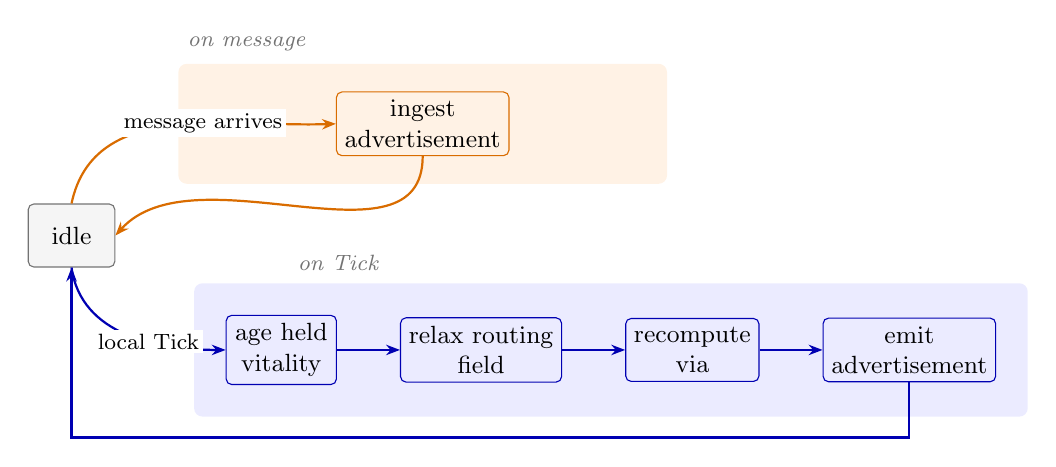
\begin{tikzpicture}[
  >={Stealth[length=5pt]},
  font=\small,
  node distance=10mm and 8mm,
  box/.style={rounded corners=2pt, draw, align=center, inner sep=3pt,
              minimum height=8mm, minimum width=14mm, text=black, fill=white},
  hub/.style={box, draw=black!55, fill=black!4, minimum width=11mm},
  recvbox/.style={box, draw=orange!85!black, fill=orange!10},
  emitbox/.style={box, draw=blue!70!black, fill=blue!8},
  recvedge/.style={draw=orange!85!black, ->, thick},
  emitedge/.style={draw=blue!70!black, ->, thick},
  elab/.style={font=\footnotesize, text=black, inner sep=1.5pt, fill=white},
  lanecap/.style={font=\footnotesize\itshape, text=black!55},
]
% --- hub (neutral, sits between the two lanes, in neither band) ---
\node[hub] (idle) {idle};

% --- top lane: reception ---
\node[recvbox, above right=6mm and 28mm of idle] (ingest) {ingest\\advertisement};

% --- bottom lane: emission ---
\node[emitbox, below right=6mm and 14mm of idle] (age) {age held\\vitality};
\node[emitbox, right=of age] (relax) {relax routing\\field};
\node[emitbox, right=of relax] (via) {recompute\\via};
\node[emitbox, right=of via] (emit) {emit\\advertisement};

% --- lane background bands (behind everything; bands DO NOT cover idle) ---
\begin{scope}[on background layer]
  \node[fill=orange!10, rounded corners=3pt, fit=(ingest),
        inner xsep=20mm, inner ysep=3.5mm] (recvband) {};
  \node[fill=blue!8, rounded corners=3pt, fit=(age)(emit),
        inner xsep=4mm, inner ysep=4mm] (emitband) {};
\end{scope}

% --- reception edges: short loop off idle (orange), the two arrows kept well apart ---
\draw[recvedge] (idle.north) to[out=78,in=182]
  node[elab, pos=0.6] {message arrives} (ingest.west);
\draw[recvedge] (ingest.south) to[out=-90,in=48,looseness=0.95] (idle.east);

% --- emission edges: long pipeline (blue) ---
\draw[emitedge] (idle.south) to[out=-82,in=180]
  node[elab, pos=0.62] {local Tick} (age.west);
\draw[emitedge] (age) -- (relax);
\draw[emitedge] (relax) -- (via);
\draw[emitedge] (via) -- (emit);
% return: drop into clear space below the band, run left, rise into idle.south
\coordinate (rdown) at ($(emit.south)+(0,-7mm)$);
\coordinate (rleft) at (idle.south |- rdown);
\draw[emitedge] (emit.south) -- (rdown) -- (rleft) -- (idle.south);

% --- lane captions: above each band's left edge, in clear space ---
\node[lanecap, anchor=south west] at ([yshift=1pt]recvband.north west) {on message};
\node[lanecap, anchor=south west] at ([xshift=12mm,yshift=1pt]emitband.north west) {on Tick};
\end{tikzpicture}
\par\vspace{1cm}
\section*{fig-forwarding}% Forwarding decision (§7.1, hand-drawn — no data). The data plane reads the RIB as a two-level policy:
% field-known? then V>=phi?. Terminals are colour-coded by valence — forward (teal, positive),
% unreachable/drop (red), not-vouched/policy (amber); decision diamonds get a light blue fill; the
% yes/no edge labels are small rounded chips so they ride the edge mid-span, never touching a box.
% Baseline tikz libraries only (arrows.meta, positioning, shapes.geometric).
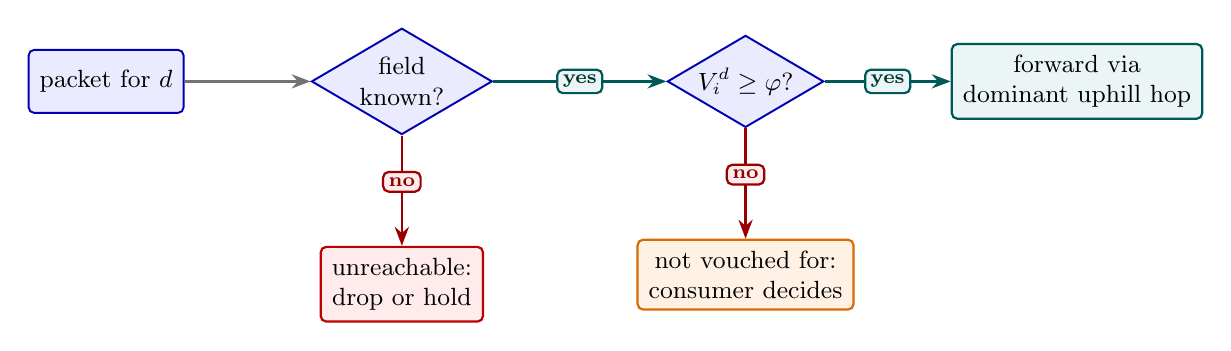
\begin{tikzpicture}[
  >={Stealth[length=2.4mm]},
  font=\small,
  node distance=10mm and 16mm,
  every node/.style={align=center},
  startnode/.style={
    rounded corners=2pt, draw=blue!70!black, fill=blue!8,
    text=black, inner sep=4pt, minimum height=8mm, line width=0.7pt},
  decision/.style={
    diamond, aspect=1.7, draw=blue!70!black, fill=blue!8,
    text=black, inner sep=1pt, line width=0.7pt},
  term/.style={
    rounded corners=2pt, text=black, inner sep=4pt,
    minimum height=8mm, line width=0.8pt},
  fwd/.style={term, draw=teal!70!black, fill=teal!8},
  drop/.style={term, draw=red!75!black, fill=red!8},
  policy/.style={term, draw=orange!85!black, fill=orange!10},
  yesedge/.style={->, draw=teal!70!black, line width=0.8pt},
  noedge/.style={->, draw=red!60!black, line width=0.8pt},
  plainedge/.style={->, draw=black!55, line width=0.8pt},
  yeschip/.style={
    fill=teal!8, draw=teal!70!black, text=teal!40!black,
    rounded corners=2pt, inner sep=2pt, font=\scriptsize\bfseries},
  nochip/.style={
    fill=red!8, draw=red!60!black, text=red!55!black,
    rounded corners=2pt, inner sep=2pt, font=\scriptsize\bfseries},
]
% --- nodes, left to right ---
\node[startnode] (pkt) {packet for $d$};
\node[decision, right=of pkt] (known) {field\\known?};

% known? --no--> drop (down), --yes--> vital (right)
\node[drop, below=14mm of known] (drop) {unreachable:\\drop or hold};
\node[decision, right=22mm of known] (vital) {$V^d_i\ge\varphi$?};

% vital? --yes--> fwd (right), --no--> policy (down)
\node[fwd, right=of vital] (fwd) {forward via\\dominant uphill hop};
\node[policy, below=14mm of vital] (policy) {not vouched for:\\consumer decides};

% --- edges ---
\draw[plainedge] (pkt) -- (known);

\draw[noedge] (known) -- node[nochip, pos=0.42] {no} (drop);
\draw[yesedge] (known) -- node[yeschip, pos=0.5] {yes} (vital);

\draw[yesedge] (vital) -- node[yeschip, pos=0.5] {yes} (fwd);
\draw[noedge] (vital) -- node[nochip, pos=0.42] {no} (policy);
\end{tikzpicture}

\end{document}
